\renewcommand{\thechapter}{\arabic{chapter}}
\setcounter{chapter}{1}

\chapter{Des propriétés physiques aux données cliniques}
\label{chap:chapter_2}
\chapterintro
Lors du précédent chapitre ont été présentés la composition et le fonctionnement de la peau ainsi que ses pathologies. De plus, une attention particulière a été portée sur l'une de ces pathologies~:~le \acrlong{lm} mais également sa forme avancée le \acrlong{lmm} et ses caractéristiques permettant son diagnostic.\par

Dans un premier temps, ce nouveau chapitre permet d'appréhender certaines propriétés physiques de la peau, notamment ses mécanismes d'interaction avec la lumière. Dans un second temps, ce chapitre évoque les principaux dispositifs optiques actuels et le type d'information mis à disposition par chacun d'entre eux pour servir le diagnostic du spécialiste. Par ailleurs, une sous-section est dédiée aux dispositifs basés sur des mesures physiques alternatives telles que l'écho d'ultrasons par exemple.\par
\newpage

\section{Propriétés de la peau}
La perception de la peau est façonnée par divers phénomènes physiques d'interaction entre la lumière et ses tissus. Ces derniers influent essentiellement de~:~
\begin{inlinerate}
    \item par leur structure, c’est-à-dire par la disposition de la matière constituant la peau,
    \item par leurs composants, c’est-à-dire par la matière elle-même.
\end{inlinerate}
Cette section est abordée de manière descendante, en déroulant le processus d'interaction d'un photon qui entre en contact avec la peau. Ce processus est schématisé de manière macroscopique sur la \Cref{fig:scheme_light_interaction}. La \textbf{réflexion spéculaire} est le premier phénomène de structure pouvant se produire à l'interface entre l'air et la peau. Par ce phénomène, la lumière incidente est réfléchie avec un angle identique à celui de la surface considérée. Ce phénomène est accentué par une peau lisse et uniforme~\cite{Yang2009}. Cette lumière est ainsi identique en matière de propriété à celle de sa source d'émission, et peut être la plupart du temps considérée comme un parasite car elle ne contient aucune information propre aux composants du milieu observé en apparaissant souvent de manière saturée sur un capteur. La \textbf{réflexion diffuse}, est un second phénomène par lequel la lumière est réfléchie dans une multitude de directions. Ce phénomène peut avoir pour origine de multiples réflexions liées à la structure du composé, ou être issu de diffractions liées au changement de propriétés du milieu~\cite{Yang2009} (coefficient de réfraction proche de celui de l'eau pour la peau). Enfin, une partie de cette lumière est perdue ou transformée selon la longueur d'onde de celle-ci~:
\begin{inlinerate}
    \item son énergie peut-être dissipée sous forme de chaleur, on parle alors de phénomène \textbf{d'absorption},
    \item ou être ré-émise avec le plus souvent une longueur d'onde différente, on parle alors de phénomène de \textbf{photoluminescence} regroupant la \textbf{fluorescence} et la \textbf{phosphorescence}~\cite{Kollias2002}.
\end{inlinerate}\par

\begin{figure}[H]
    \centering
    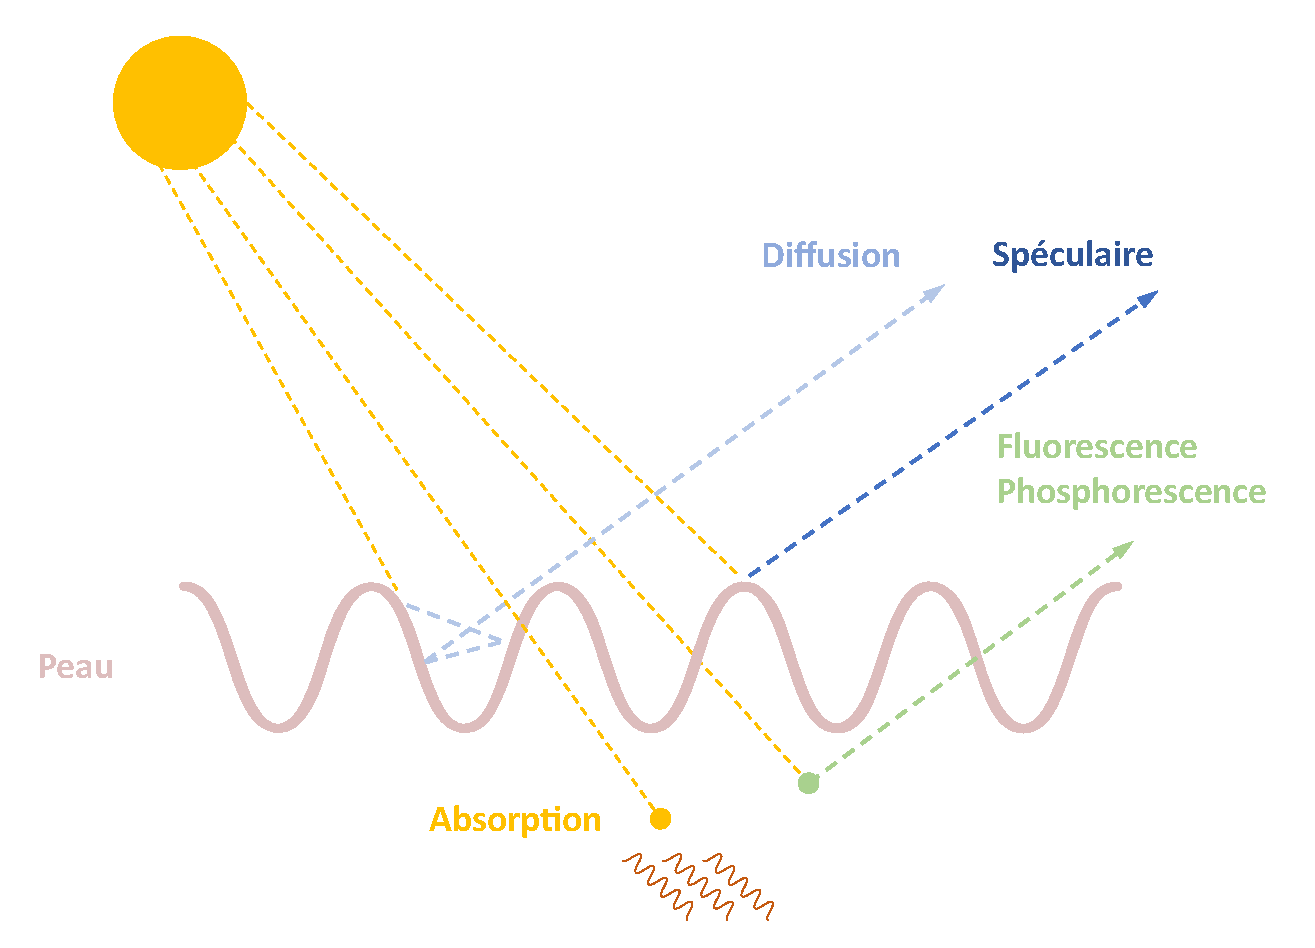
\includegraphics[width=\linewidth]{contents/chapter_2/resources/scheme_light_interaction.pdf}
    \caption{Schéma représentant les principaux mécanismes d'interaction qui peuvent survenir suite à l'interaction de la lumière avec la peau. Les modalités optiques tentent d'exploiter ces divers phénomènes pour extraire une information sur les tissus analysés.}
    \label{fig:scheme_light_interaction}
\end{figure}\par

Dans cette configuration, le choix de la source d'émission de lumière est l'un des points importants. En effet, comme démontré dans un travail précédent employant le principe de la \gls{del} en dermatologie~\cite{Barolet2008}, \textbf{la longueur d'onde d'émission} est l'un des paramètres d'influence possible quant à la profondeur des structures à observer dans la peau. Ainsi, des longueurs d'onde à l'entrée du spectre visible humain ($\approx$\SI{380}{\nano\metre}) ne parviennent pas à se frayer un chemin en profondeur et ne frôlent que les couches supérieures de l'épiderme, tandis que des longueurs d'onde plus élevées de ce même spectre ($\approx$\SI{780}{\nano\metre}) tendent à atteindre l'hypoderme et ses vaisseaux sanguins. Une synthèse de la pénétration de la lumière en fonction de la longueur d'onde est visible sur la \Cref{fig:scheme_light_penatrating}.\par

\begin{figure}[H]
    \centering
    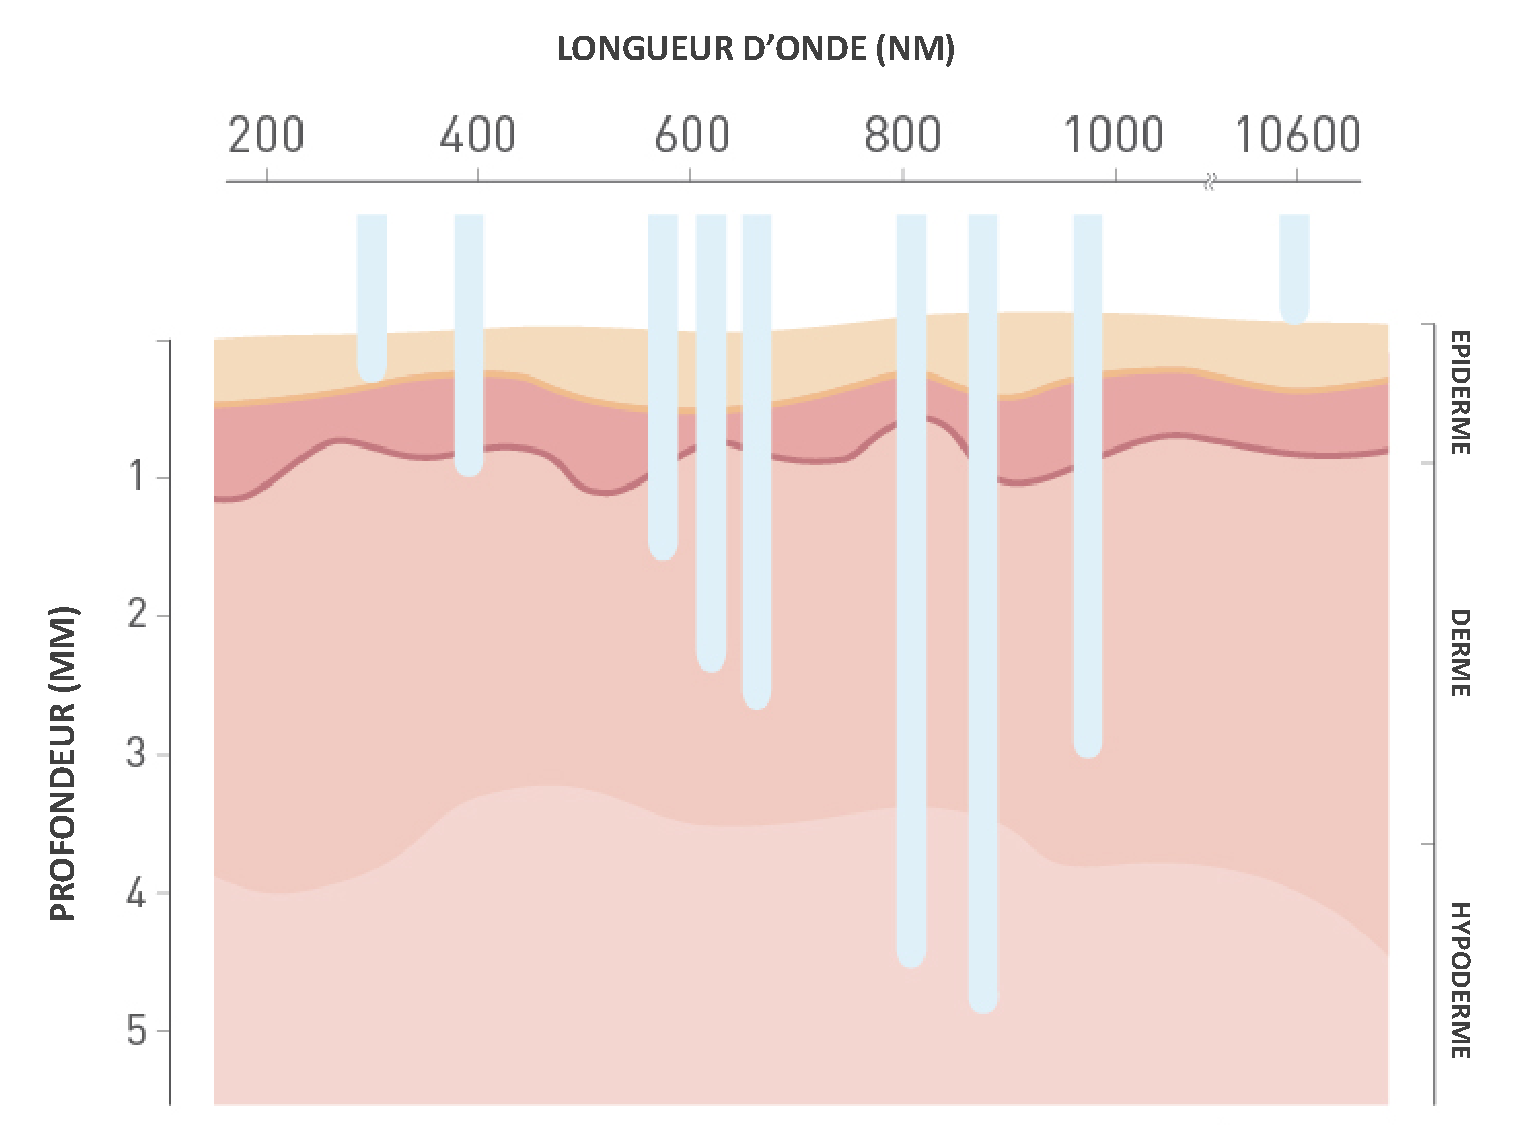
\includegraphics[width=0.95\linewidth]{contents/chapter_2/resources/scheme_light_penatrating.pdf}
    \caption{Schéma représentatif de la profondeur de pénétration (en mm) de la peau en fonction de la longueur d’onde de la lumière~\cite{Barolet2008}. Il s'agit d'un ordre de grandeur moyen constaté chez l'être humain, les propriétés de la peau variant d'un emplacement à un autre. Aucune information relative aux types de peaux étudiés, selon l'échelle de Fitzpatrick par exemple, n'a été mentionnée.}
    \label{fig:scheme_light_penatrating}
\end{figure}\par

Outre la question de la profondeur, le choix de la longueur d'onde permet d'\textbf{interagir avec différents types de chromophores} et permet de renseigner localement sur des propriétés de la peau. Certains travaux focalisés sur les systèmes lasers et d'émission en général~\cite{Stewart2013} ont permis de mettre en avant le rapport entre la longueur d'onde et des composants majeurs de la peau tels que \textbf{l'eau, l'hémoglobine (oxygénée ou non) ou la mélanine}. Pour illustrer ce propos, la \Cref{fig:scheme_light_absorption} synthétise ce rapport entre la longueur d'onde d'émission et l'absorption associée aux principaux composants chromophores de la peau dont les quatre mentionnés. La quantification de ces composants peut présenter un intérêt dans la mesure où certaines pathologies peuvent altérer le métabolisme et donc modifier fondamentalement le ratio de chromophores présents, pouvant par exemple amener à une hypervascularisation. Certains travaux tentent ainsi de revenir à des fonctions de métabolisme~\cite{Im2016}.\par

\begin{figure}[H]
    \centering
    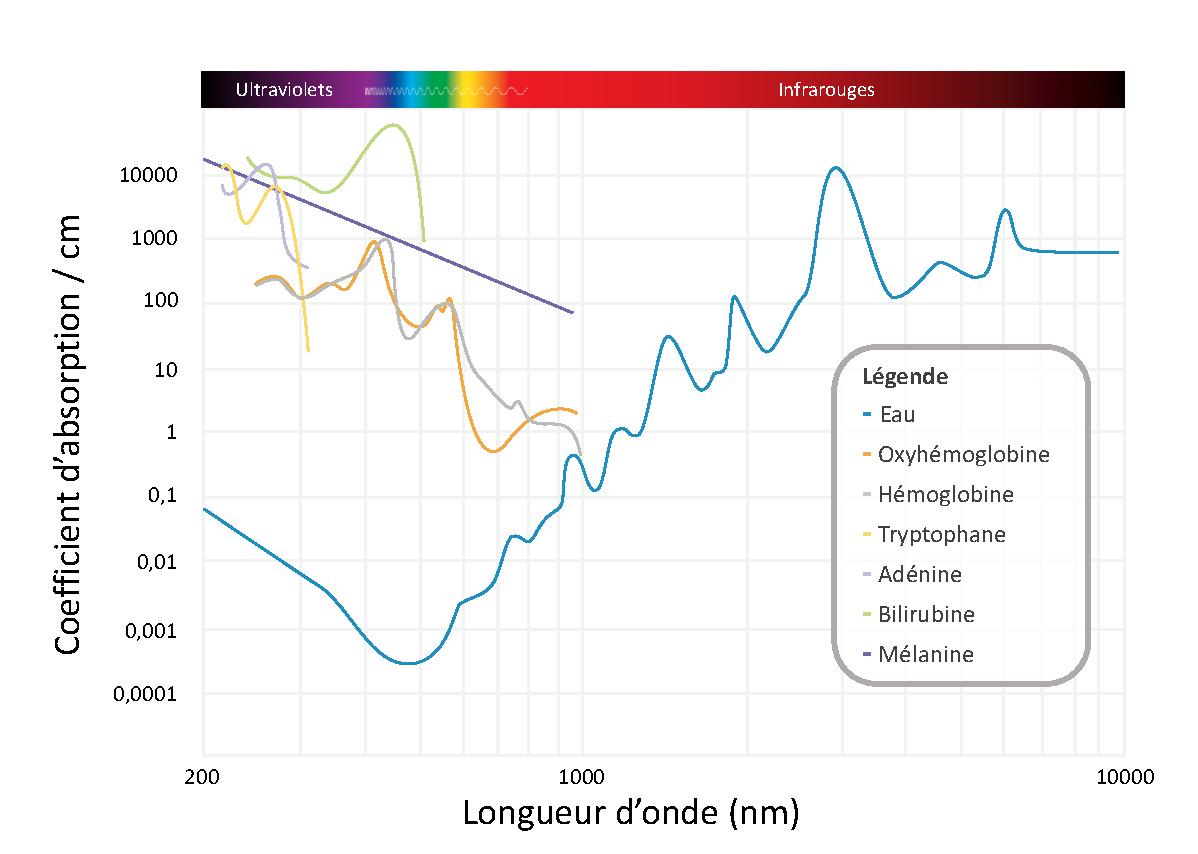
\includegraphics[width=\linewidth]{contents/chapter_2/resources/scheme_light_absorption.pdf}
    \caption{Représentation des coefficients d'absorption en fonction de la longueur d'onde pour les principaux composants chromophores présents dans la peau~\cite{Raulin2013}.}
    \label{fig:scheme_light_absorption}
\end{figure}
 
\clearpage

\section{Modalités d’imagerie non-invasives}
Pour le diagnostic et aussi afin de mieux suivre, voire de conserver une trace de leurs patients, les dermatologues disposent de nombreux outils. Ils peuvent entre autres dans leur pratique clinique se référer à divers types d’examens, distingués dans ce travail sous deux catégories~:
\begin{itemize}
    \item d’une part \textbf{les examens non-invasifs}, c’est-à-dire ne provoquant pas de destruction des tissus du corps humain. Ces dispositifs sont capables de restituer une image différente des tissus selon la nature du phénomène physique observé et ne provoquent en général pas d’inconfort particulier pour le patient. Ils peuvent représenter un investissement initial important mais s'amortissent assez bien sur le long terme. 
    \item d’autre part \textbf{les examens invasifs}, c’est-à-dire provoquant une effraction des tissus. L'histopathologie est le principal mode d'examen invasif et représente à ce jour le \textit{gold standard} de ce domaine. Cet examen se réalise par biopsie, c’est-à-dire par prélèvement de tissus puis par une analyse histologique de ceux-ci. Cette technique peut être incommodante pour le patient et requiert plus de temps qu'un examen non-invasif et est généralement plus coûteuse à l'unité.
\end{itemize}\par

Après avoir présenté de manière non exhaustive les principales pathologies de la peau et les principes d'interaction majeurs de la lumière avec cet organe, il convient désormais d'aborder les diverses méthodes permettant une observation non-invasive. Ces modalités d'imagerie franchissent en majorité le cap du numérique permettant un suivi plus aisé, voire un échange plus rapide entre professionnels, et l’utilisation de traitements automatiques. À nouveau, deux catégories distinctes sont utilisées pour séparer ces techniques avec d’une part \textbf{les techniques de mesure optique} et d'autre part \textbf{les techniques de mesure non-optique} basées sur divers phénomènes physiques quantifiables.\par

\subsection{Modalités par mesure optique}
Cette partie décrit les principaux appareils existants permettant l'observation de la peau. Évidemment, ces modalités sont également transposables à d'autres domaines d'application que celui de la dermatologie. Les dispositifs méconnus ou expérimentaux encore loin d'une application clinique ne sont pas présentés dans cette sous-section. La \Cref{tab:light_absorption} met en lumière ces dispositifs et leurs caractéristiques générales à but indicatif.\par

\begin{table}[H]
\begin{tabular}{lllll}
    \toprule
    \textbf{Technologie}                        & \textbf{Effet}    & \textbf{Résolution Spatiale} & \textbf{Profondeur}                \\ \hline
    Imagerie clinique                           & Réflectance       & Lentille dépendant           & \SIrange{0.1}{1}{\milli\metre}     \\
    Dermatoscopie                               & Réflectance       & Lentille dépendant           & \SIrange{0.1}{1}{\milli\metre}     \\
    Microscopie confocale par réflectance       & Réflectance       & \si{\micro\metre}            & \textless{} \SI{200}{\micro\metre} \\
    Tomographie en cohérence optique            & Réflectance       & \si{\micro\metre}            & \SIrange{1}{2}{\milli\metre}       \\
    Imagerie multispectrale                     & Réflectance       & Lentille dépendant           & \SIrange{0.1}{1}{\milli\metre}     \\
    Spectroscopie à réflexion                   & Réflectance       & Diamètre de la fibre         & \SIrange{0.1}{1}{\milli\metre}     \\
    Microscopie confocale Raman                 & Raman             & \si{\micro\metre}            & \SI{150}{\micro\metre}             \\
    \bottomrule
\end{tabular}
\caption{Table des principales modalités de mesure optique utilisées à but clinique ou à un stade de recherche clinique en dermatologie~\cite{Kollias2002}.}
\label{tab:light_absorption}
\end{table}\par

\subsubsection{Imagerie clinique}
L’examen de dépistage classique est associé en dermatologie à une inspection à l’œil nu exercée par une personne compétente ou sensibilisée à la détection de pathologies. L'\textbf{imagerie clinique} fait appel à un dispositif de photographie non propre à la dermatologie. Par ailleurs, elle constitue historiquement la première modalité de cette discipline mais également la moins onéreuse car emploie des caméras non spécifiques à la discipline.\par

Avant l’avènement de l’informatique, cette modalité se basait sur des supports de type argentique. L’évolution de ce matériel vers le numérique, et l’arrivée de systèmes de type \gls{pacs} ont conjointement motivé une transition vers des données dématérialisées.\par

Ce type d’imagerie donne à l’observateur un point de vue subjectif, similaire à une observation à l’œil nu, utile dans le cadre d’un diagnostic à distance ou dans le suivi à long terme d’un patient. Néanmoins, les principaux points faibles sont \textbf{le manque de standard concernant le format d'image} et \textbf{le manque de protocole concernant l'acquisition des images}~:~pas de spécifications d'éclairage, ni même de spécifications sur le point de vue à adopter au moment de la prise d'image.\par

Ces dernières années ont vu l'émergence de nouveaux types de dispositifs qui étendent la photographie clinique au corps entier. Ces appareils permettent une traçabilité et un suivi des lésions apparentes sur le corps d'un patient. En effet, l'un des meilleurs critères du suivi des lésions dans le dépistage de pathologies telles que le mélanome, reste le suivi de leur évolution au cours du temps. Cet élément a notamment été mis en avant en 2004, et est encore considéré au moment de cette rédaction comme l'un des critères majeurs~\cite{Abbasi2004,Glazer2017}. Différents industriels commercialisent des dispositifs de plus en plus performants dont FotoFinder et son système ATBM mais également la société Pixience avec le Body-Mapper® permettant ce suivi ainsi qu'un contrôle de l'éclairage lors de la prise de vue. Une interface guide le médecin lors de la prise d'images et permet d'associer à un modèle humain les diverses parties du corps (voir la \Cref{fig:example_device_bodymapper}).\par

\begin{figure}[H]
\centering
    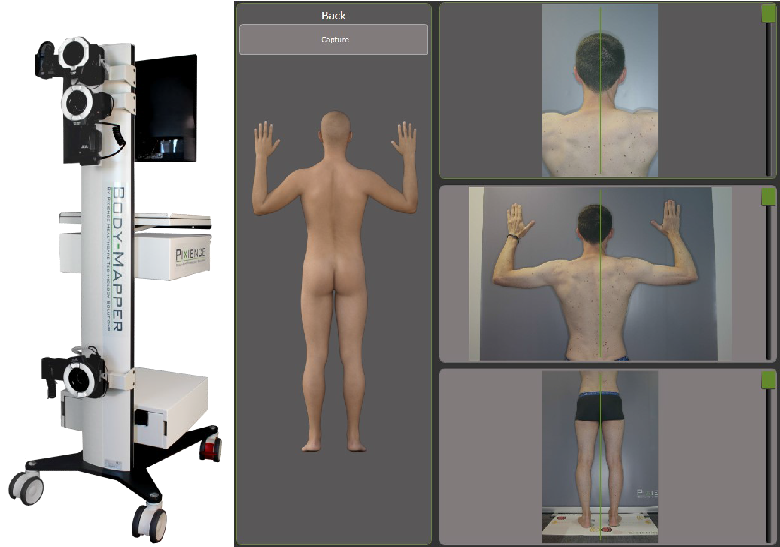
\includegraphics[width=0.75\linewidth]{contents/chapter_2/resources/example_device_bodymapper.pdf}
    \caption{Exemple du Body-Mapper, un appareil de photographie clinique corps entier, proposé par Pixience. À gauche, l'appareil d'acquisition ; À droite, son interface logicielle permettant d'acquérir les diverses parties du corps.}
    \label{fig:example_device_bodymapper}
\end{figure}\par

\subsubsection{Dermatoscopie}
Également appelé \textit{dermoscopie}, \textit{microscopie en épiluminescence} ou encore \textit{microscopie de surface}, ce dispositif permet d’observer les lésions cutanées. Le terme de \textbf{dermatoscopie} est préféré aux autres pour la suite de ce manuscrit. Cette technique d’imagerie est partiellement attribuée à Johan Christophorus Kohlhaus dont les travaux menés au \siecle{17}, auraient grandement contribué à initier cette modalité. Les premiers dispositifs ont émergé en 1971~\cite{MacKie1972}, et ce sont les années 1980 qui ont contribué à son essor chez un grand nombre de praticiens.\par

Cet outil possède comme première caractéristique, \textbf{de réduire les réflexions de lumière et contribue à rendre le stratum corneum translucide}~\cite{Katz2001}, permettant ainsi au praticien de visualiser les couches sous-jacentes~:~épiderme, \gls{jde} ou encore le derme papillaire non visible à l’œil nu. Cette réflexion de lumière était initialement supprimée par l’utilisation d’un fluide (eau, gel, \ldots) entre la peau et la lentille du dispositif (dermatoscope non polarisé). De récentes améliorations ont permis \textbf{de rendre l'utilisation d'un fluide obsolète par l'utilisation de lumière polarisée} (dermatoscope polarisé). Un premier filtre polarisé orienté dans une direction est disposé juste après la source de lumière, puis un second filtre polarisé perpendiculairement au premier filtre est mis en place avant la fenêtre d'observation (voir \Cref{fig:scheme_polarized_dermoscopy}). Ce dispositif permet ainsi de s'affranchir de la lumière spéculaire directement issue de la source de lumière qui parasite l'observation~\cite{CamposdoCarmo2008}.\par

\begin{figure}[H]
\centering
    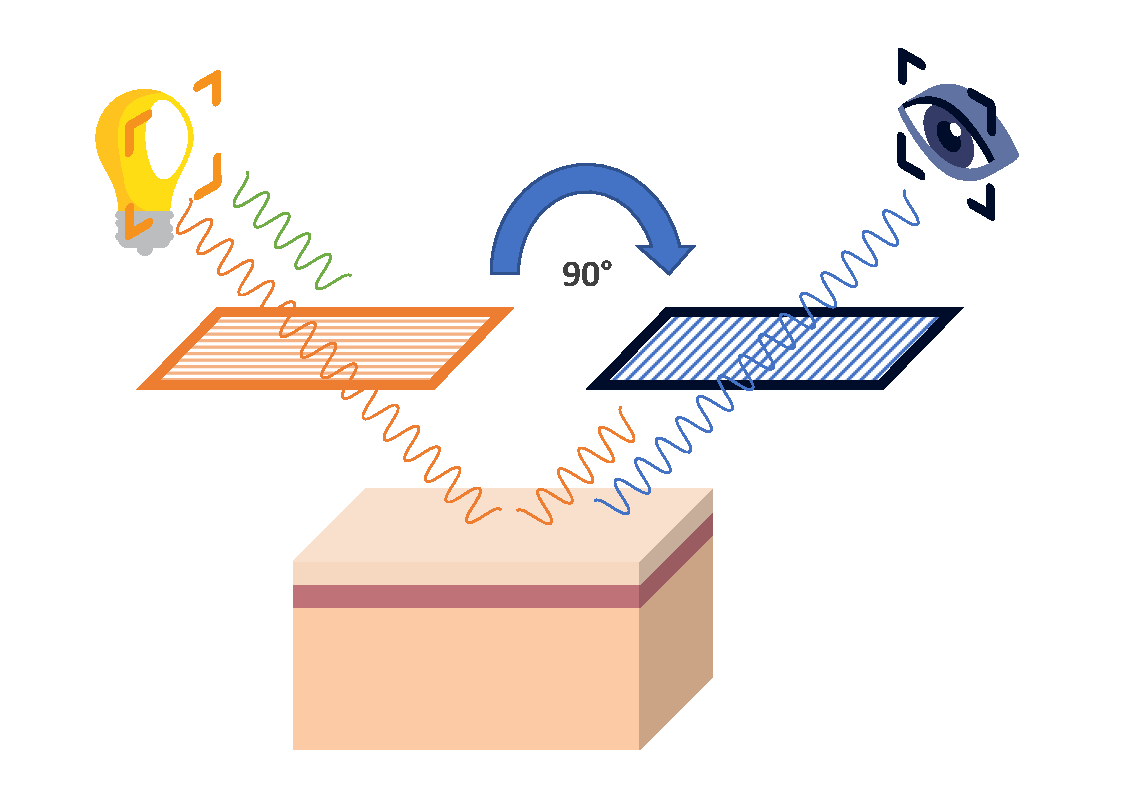
\includegraphics[width=0.85\linewidth]{contents/chapter_2/resources/scheme_polarized_dermoscopy.pdf}
    \caption{Principe de la dermatoscopie à lumière polarisée. Un premier filtre polarisé est disposé après la source de lumière, puis un second filtre dont la polarisation est perpendiculaire au premier est disposé juste avant la fenêtre d'observation~\cite{sonthalia2019}.}
    \label{fig:scheme_polarized_dermoscopy}
\end{figure}\par

Une seconde caractéristique non négligeable de ce dispositif, est la mise à disposition d’un zoom permettant de grossir en lumière blanche jusqu'à 400 fois selon la complexité des modèles proposés~\textsuperscript{\ref{footnote:medicam}}. Cette dernière caractéristique octroie au praticien la possibilité d’appréhender au mieux la structure de la peau dans ses moindres détails~\cite{CamposdoCarmo2008}.\par

\addtocounter{footnote}{1}
\footnotetext[\thefootnote]{Source~:~\href{https://www.fotofinder.de/fr/technologie/diagnostic-du-cancer-de-la-peau/medicam/}{FotoFinder medicam 1000s}. \label{footnote:medicam}}

De plus, son faible coût d’achat, sa rapidité de diagnostic et son efficacité face au seul œil humain contribuent largement à sa démocratisation dans la profession~\cite{Lallas2013}. Bien que cette modalité soit utilisée majoritairement dans le dépistage de \textit{lésions pigmentées}, son efficacité semble avérée dans le cas de \textit{lésions non pigmentées} telles que le \gls{cbc} et le \gls{csc}~\cite{Lallas2013}.\par

Ces dispositifs tendent à s'adapter de plus en plus aux besoins de leur marché, en proposant par exemple une caméra haute résolution et permettant une utilisation polyvalente de l'appareil avec un connecteur générique comme le propose la société \textit{Pixience} (voir la \Cref{fig:example_device_ccube}). L'utilisation de cet appareil dans certaines études, a permis la mise en avant de pathologie de la peau chez la souris~\cite{Pillon2017} et chez l'homme~\cite{Cinotti2016}. Certaines sociétés comme \textit{DermLite}, proposent une solution plus nomade et adaptable aux principaux dispositifs de photographie du marché. La solution \textit{DL3N} est visible sur la \Cref{fig:example_device_dermlite}.\par

\begin{figure}[H]
    \centering
    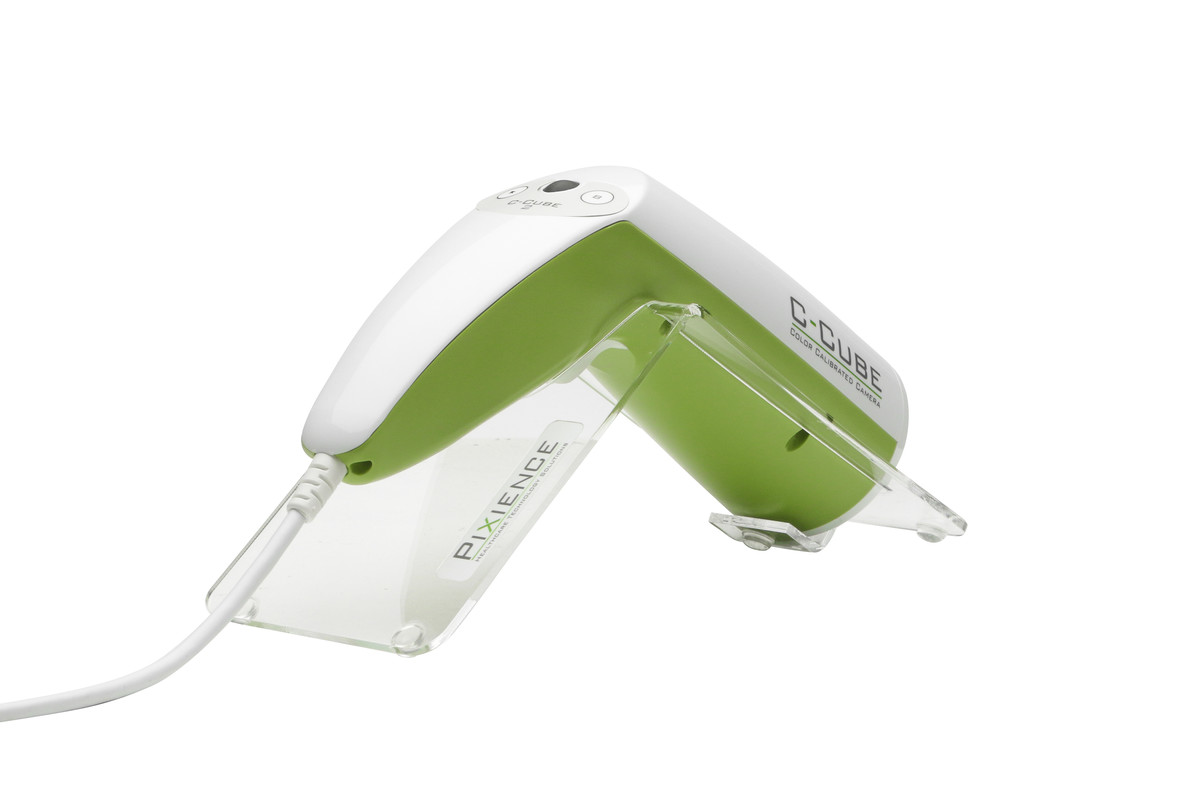
\includegraphics[width=0.75\linewidth]{contents/chapter_2/resources/example_device_ccube.jpg}
    \caption{Exemple du dispositif de dermatoscopie \textit{C-Cube} proposé par la société \textit{Pixience}.}
    \label{fig:example_device_ccube}
\end{figure}\par

\begin{figure}[H]
\centering
    \begin{subfigure}{.32\textwidth}
      \centering
      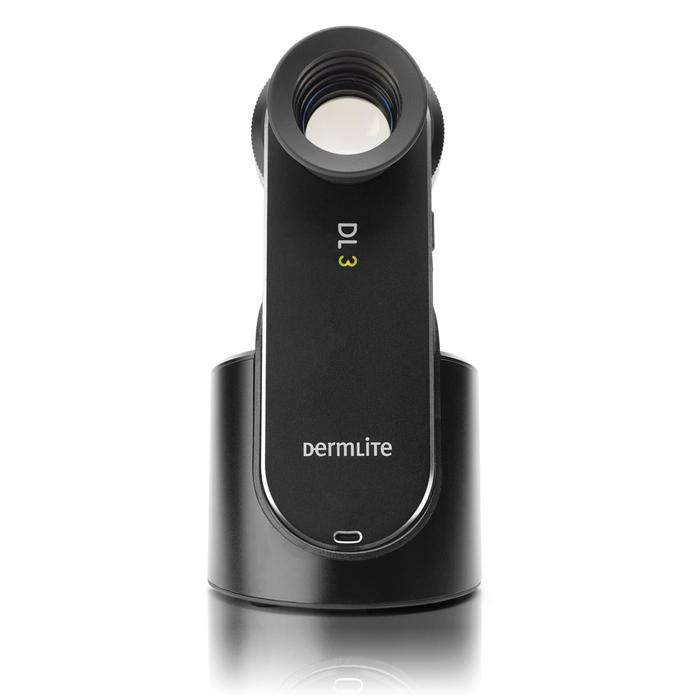
\includegraphics[width=\linewidth]{contents/chapter_2/resources/example_device_dermlite_1.png}
    \end{subfigure}
    \begin{subfigure}{.32\textwidth}
      \centering
      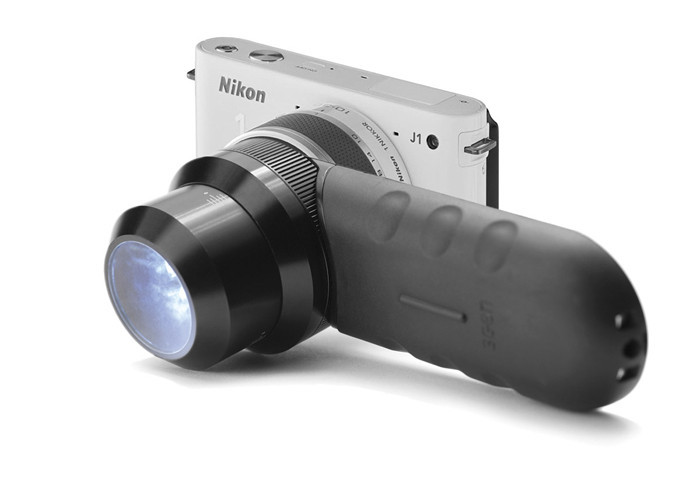
\includegraphics[width=\linewidth]{contents/chapter_2/resources/example_device_dermlite_2.png}
    \end{subfigure}
    \begin{subfigure}{.32\textwidth}
      \centering
      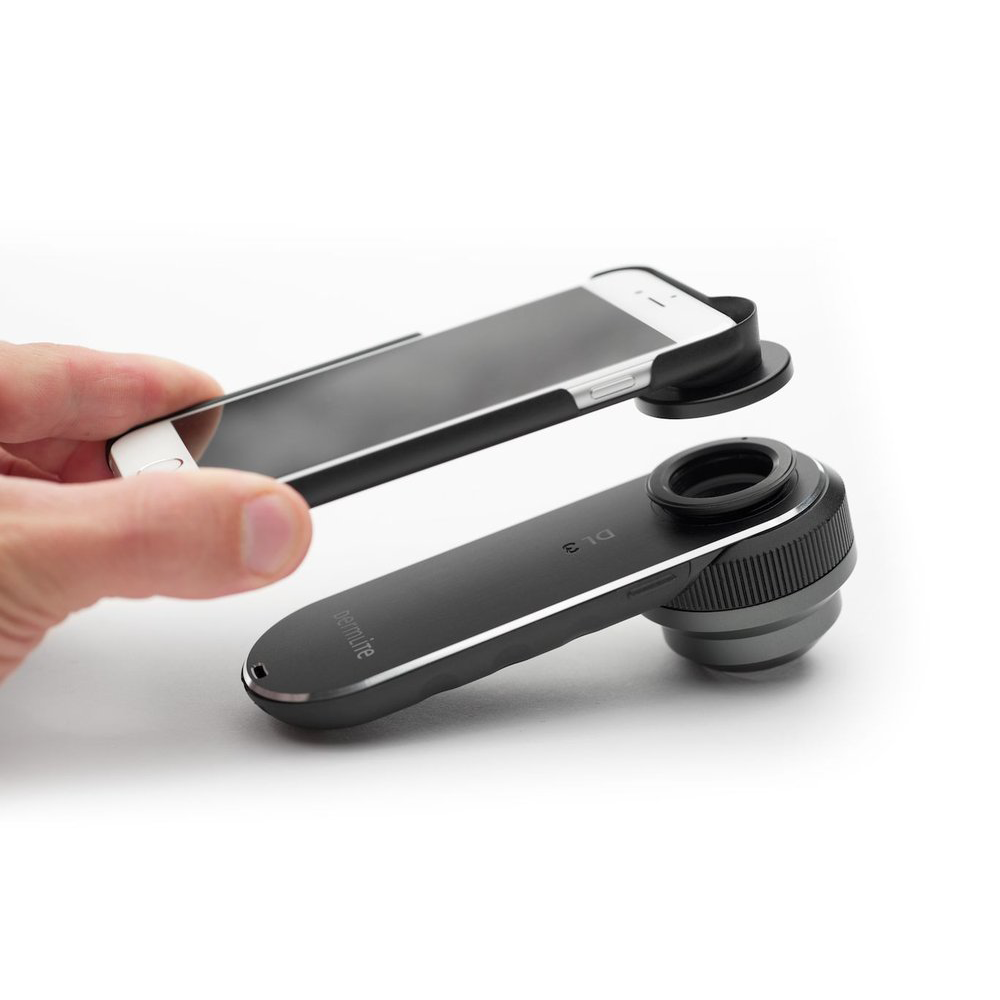
\includegraphics[width=\linewidth]{contents/chapter_2/resources/example_device_dermlite_3.png}
    \end{subfigure}
    \caption{Exemple du dispositif de dermatoscopie \textit{DL3N} proposé par la société \textit{DermLite}. À gauche, le dispositif seul ; Au milieu, ce même dispositif adapté à un appareil photo standard ; À droite, le dispositif adapté à une caméra de téléphone portable.}
    \label{fig:example_device_dermlite}
\end{figure}\par

\subsubsection{Microscopie confocale par réflectance}
La \textbf{\acrfull{mcr}} est une technique d’imagerie décrite durant les années 1950 par Marvin Minsky~\cite{Sheppard2015}. Les avancées réalisées durant les années 1990 ont permis de réduire considérablement la taille de cet appareil et de faciliter ainsi son utilisation dans divers domaines. Cette technique de plus en plus répandue dans les services de dermatologie a également connu un regain de notoriété dans les journaux scientifiques~:~une recherche à l’aide des mots-clés « reflectance confocal microscopy skin » apporte une dizaine de publications vers les années 2000 contre une moyenne de 1500 chaque année depuis 2010~\textsuperscript{\ref{footnote:scholar_rcm}}.\par

\addtocounter{footnote}{1}
\footnotetext[\thefootnote]{Source~:~Google Scholar. \label{footnote:scholar_rcm}}

Cette technique emploie l’utilisation d’un \textit{sténopé} situé devant le capteur et permet \textbf{de conserver uniquement les photons issus d'un plan focal}, illustré en \Cref{fig:scheme_principle_rcm}. Ce principe octroie la possibilité \textbf{d'ajuster la profondeur} de ces \textit{plans focaux} ou \textit{plans de coupes}, permettant l'acquisition d'images à une même profondeur ou l'acquisition de «piles» d'images dont la profondeur varie~\cite{Sheppard2015}. En dermatologie, les dispositifs se basent sur des longueurs d’onde de \SI{830}{\nano\metre} non-invasives pour la peau et les yeux, mais limitent la profondeur du dispositif à \SIrange{200}{300}{\micro\metre}.\par

\begin{figure}[H]
\centering
    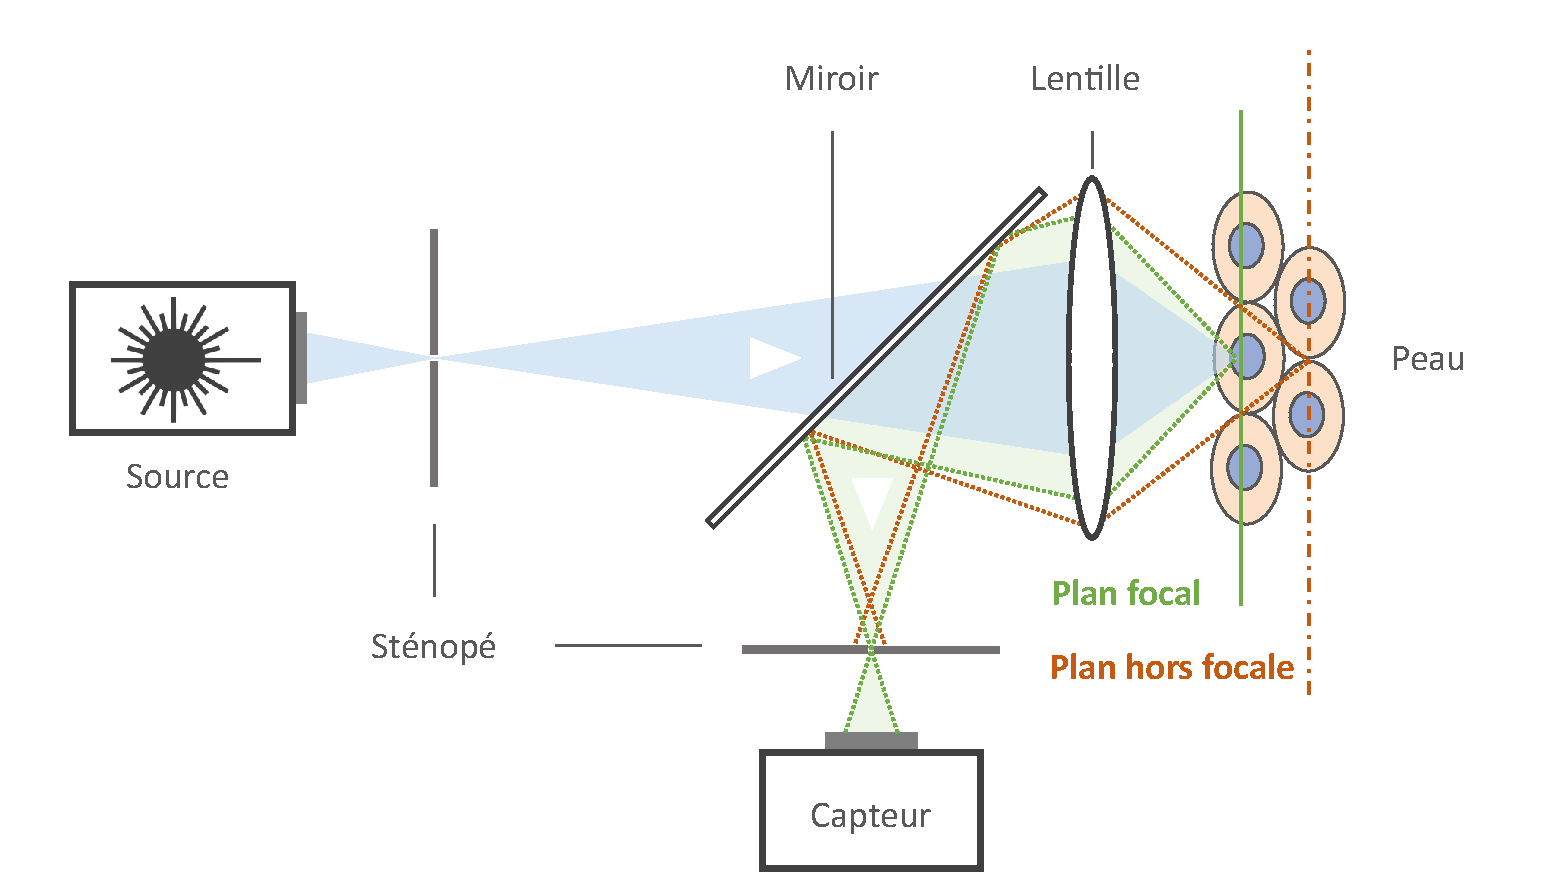
\includegraphics[width=\linewidth]{contents/chapter_2/resources/scheme_principle_rcm.pdf}
    \caption{Schéma de fonctionnement du \gls{mcr} par Marvin Minsky. Une source de lumière est émise et focalisée en un point spécifique de la peau puis la lumière est réfléchie et reçue par une caméra au travers d'un sténopé (trou de faible diamètre). La lumière réfléchie en dehors du plan focal défini par l'utilisateur est ainsi arrêtée par ce sténopé.}
    \label{fig:scheme_principle_rcm}
\end{figure}\par

Enfin, à la manière du dermatoscope, un gel à base d’eau de réfraction proche de celle de l’épiderme est utilisé entre la lentille du dispositif et la peau afin de limiter la perte de photons et de permettre l’obtention d’images du derme.\par

\subsubsection{Tomographie en cohérence optique}
Initialement conçue pour le domaine de l’ophtalmologie, la \gls{tco} est une technique récente qui se base sur le principe d’interférométrie et qui tend à se démocratiser à de nombreux domaines d’intervention dont celui de la dermatologie. Schématisé sur la \Cref{fig:scheme_principle_oct}, ce principe consiste à utiliser \textbf{une source de lumière commune divisée en deux faisceaux}, le \textbf{premier servant de référence} et le \textbf{second servant à l’analyse de l’échantillon}. Ainsi, le faisceau de référence va transiter via un chemin contenant un miroir ajustable permettant de modifier sa distance parcourue. En modifiant cette distance, la profondeur désirée va pouvoir être ajustée au sein de l'échantillon à analyser. En effet, lors de la superposition des deux faisceaux à l'entrée du récepteur, une \textit{interférence constructive} est observée lorsque l'information est en phase, cette information est alors \textbf{amplifiée}, tandis qu'une \textit{interférence destructive} est observée lorsque l'information est en déphasage, cette information est alors \textbf{atténuée}.\par

Initialement, ce principe a été exploité pour des dispositifs dits d’interférométrie à faible cohérence temporelle et fournissait une information à une dimension. La \gls{tco} est une extension de ce principe à deux dimensions, permettant la caractérisation d’une \textit{tranche} de tissu. Cette modalité d’imagerie propose ainsi une information temps réel en profondeur (de l’ordre du millimètre), avec une résolution proche du micromètre. Par ailleurs, il est possible d'obtenir une reconstruction de la peau et de ses structures, par l'acquisition de plusieurs plans de coupe.\par

\begin{figure}[H]
    \centering
    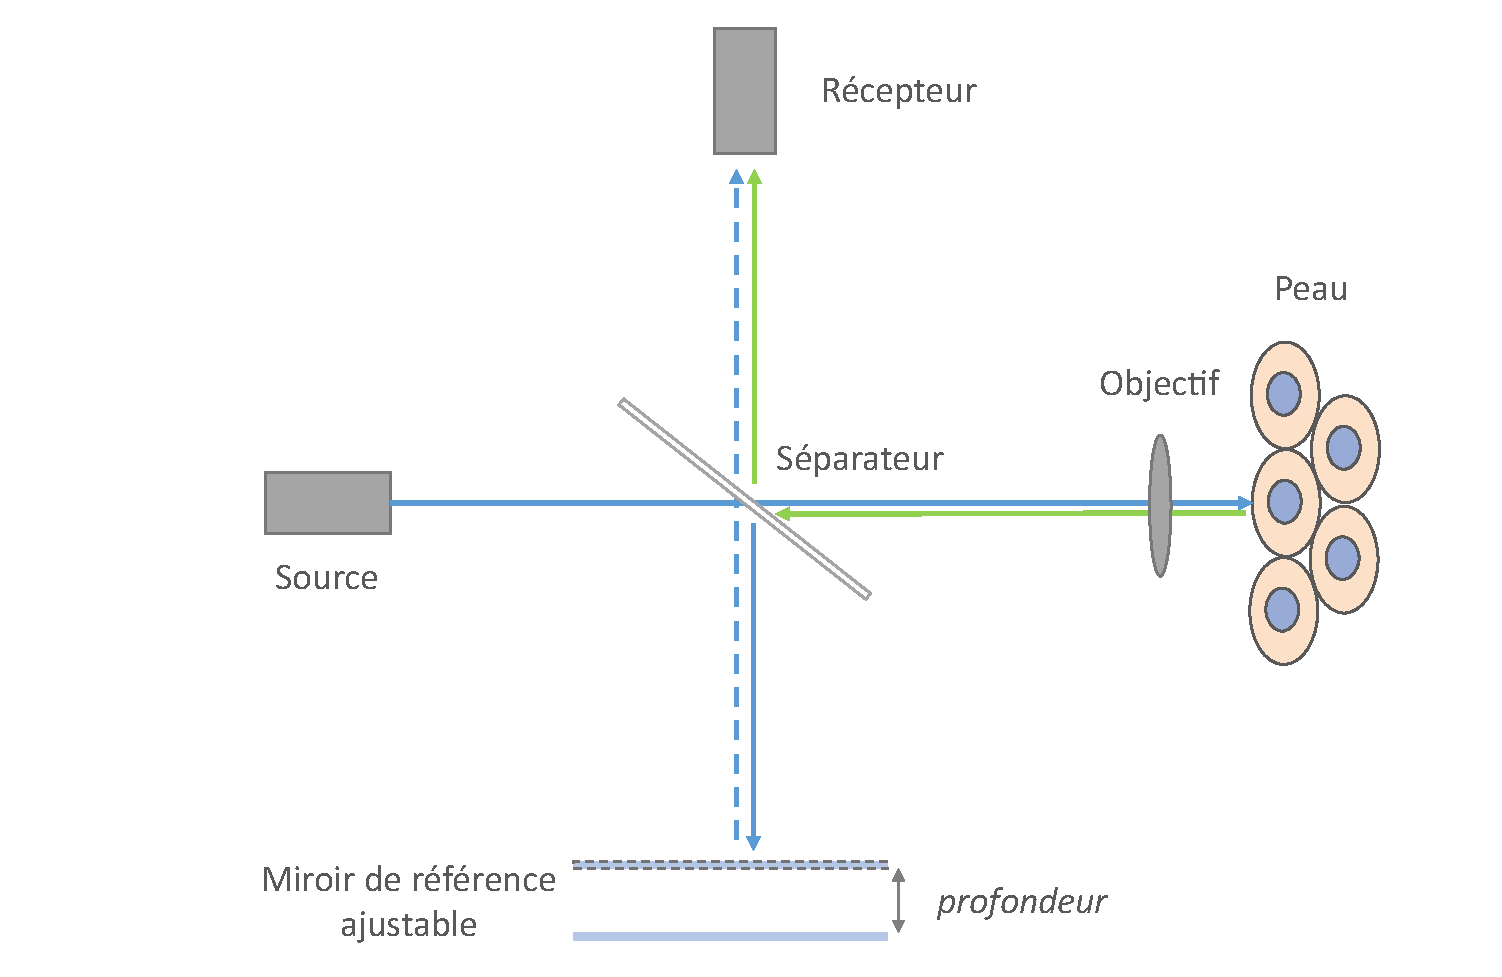
\includegraphics[width=1\linewidth]{contents/chapter_2/resources/scheme_principle_oct.pdf}
    \caption{Schéma de fonctionnement de la \gls{tco}. Une source de lumière génère un unique faisceau divisé en deux faisceaux identiques. L'un de ces faisceaux résultants sert de signal de référence (en bleu), tandis que le second sert à l'analyse de l'échantillon (en vert). Par la suite, ces deux faisceaux sont recombinés à l'entrée du récepteur.}
    \label{fig:scheme_principle_oct}
\end{figure}\par
\clearpage

\subsubsection{Spectroscopie par réflectance}
La spectroscopie de réflectance fournit une information de spectre à un même instant, c’est-à-dire contenant plusieurs valeurs numériques, chacune propre à une longueur d'onde spécifique. L'information fournie est propre à un unique point de l'espace et est obtenue en temps réel. Ainsi, cette modalité ne constitue pas une technique d'imagerie au sens matriciel à deux dimensions.\par

Pour cela, une source de lumière uniforme et stable dans le temps est utilisée, mais également couvrant l'ensemble du spectre désiré. Cette lumière est ensuite canalisée au sein d'une ou plusieurs fibres optiques afin d'être conduite jusqu'à l'échantillon supposé. Le phénomène de réflectance de l'échantillon est ensuite capté à l'aide d'une ou plusieurs fibres optiques jusqu'à un spectromètre qui va dissocier le signal (phénomène de diffraction), afin de cibler de multiples cellules présentes sur un capteur numérique~\cite{Murphy2005,Mallia2008}\textsuperscript{\ref{footnote:aventes_spectrometer}}.\par

Ces capteurs font l'objet d'une procédure de calibration à l'aide de \textit{pantones} ou nuanciers dont les propriétés visuelles sont établies, comme le propose par exemple le ColorChecker\textsuperscript{®}~\textsuperscript{\ref{footnote:colorchecker}}. En effet, il est nécessaire d'empêcher une saturation du signal conduisant à une perte d'information tout en exploitant au mieux la quantification octroyée par le capteur. Sa nécessité est le fruit des multiples conditions d'éclairage possibles de l'environnement mais également de la variété des sources de lumière pouvant être employées avec ce type de dispositif. Cette étape de calibration permet de rectifier et compenser le signal obtenu par le capteur, et d'obtenir une version \textit{idéale} de celui-ci dont l'information est maximisée.\par

\begin{figure}[H]
    \centering
    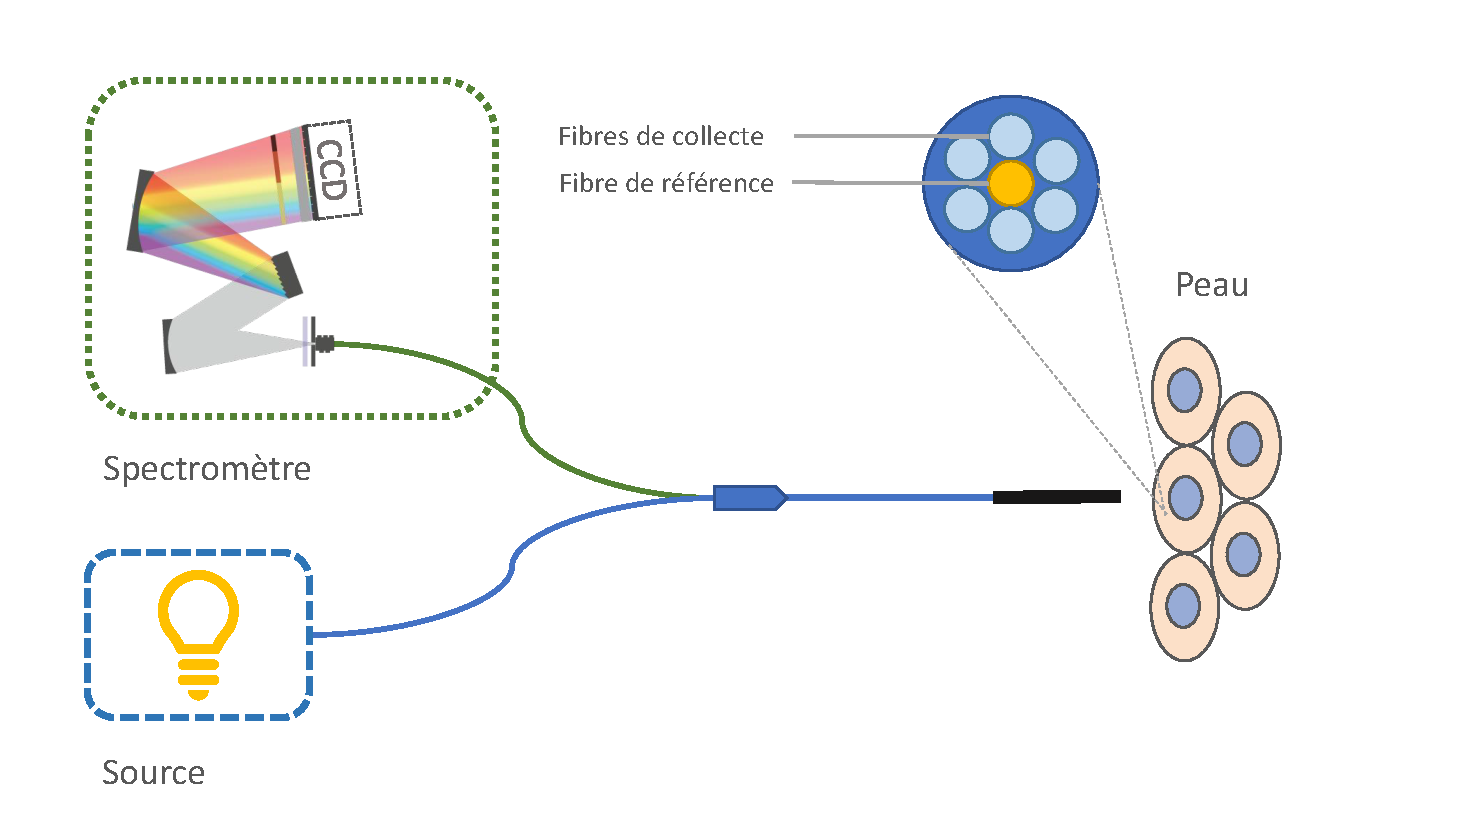
\includegraphics[width=\linewidth]{contents/chapter_2/resources/scheme_principle_spectroscopy.pdf}
    \caption{Schéma représentant le fonctionnement d'un spectroscope par réflectance. Une lumière de référence est générée puis acheminée jusqu'à la zone cible. Cette lumière transite le long d'une ou plusieurs fibres optiques. Puis le phénomène de réflectance est capté et envoyé au spectromètre par le biais d'une ou plusieurs fibres. Le signal reçu est ensuite décomposé puis envoyé à la surface d'un capteur numérique.}
    \label{fig:scheme_principle_spectroscopy}
\end{figure}\par

\addtocounter{footnote}{1}
\footnotetext[\thefootnote]{Source~:~Spectromètres AvaSpec\textsuperscript{®}, Avantes, Pays-Bas. \label{footnote:aventes_spectrometer}}

\addtocounter{footnote}{1}
\footnotetext[\thefootnote]{Source~:~X-Rite, ColorChecker\textsuperscript{®}, Michigan, États-Unis. \label{footnote:colorchecker}}

\subsubsection{Imagerie multispectrale}
L'imagerie multispectrale est l'extension spatiale de la spectroscopie et l'extension spectrale de l'imagerie clinique. Par ce principe d'imagerie, les pixels contenus dans une image ne se résument pas à une valeur pour les images en intensités de gris ou à trois valeurs pour des images RGB, mais à une multitude de valeurs décrivant chacune une longueur d'onde. Ce nombre de valeurs spectrales est ainsi dépendant de la précision recherchée dans un domaine d'application particulier. Les temps d'acquisition entre les diverses valeurs tendent à se réduire fortement avec les évolutions technologiques. Différents principes sont mis en oeuvre pour parvenir à l'obtention de ces images, visible sur la \Cref{fig:scheme_multispectral_principle}. Ce travail retient les principes suivants~:
\begin{itemize}
    \item par modification \textbf{de la source émettrice de lumière}, soit en utilisant des \gls{del} programmables, des lasers ou encore des combinaisons de filtres permettant de modifier les propriétés de la lumière,
    \item par filtrage \textbf{de la lumière reçue}, bien souvent à l'aide de combinaisons de filtres permettant de choisir les longueurs d'onde désirées. Des capteurs multicouches ont émergé ces dernières années et permettent une acquisition quasiment simultanée de l'information sur le capteur en lui-même~\textsuperscript{\ref{footnote:foveon_sensor}}.
\end{itemize}\par

Ce principe permet de proposer une information plus riche que celle transmise par les capteurs habituels du marché. Ces appareils permettent de mettre cette information en relation avec des modèles d'absorption et de remonter à une estimation de la composition et de la structure du tissu.\par 

\addtocounter{footnote}{1}
\footnotetext[\thefootnote]{Source~:~Foveon X3®, Foveon, Santa Clara, Californie. \label{footnote:foveon_sensor}}

\begin{figure}[H]
    \centering
    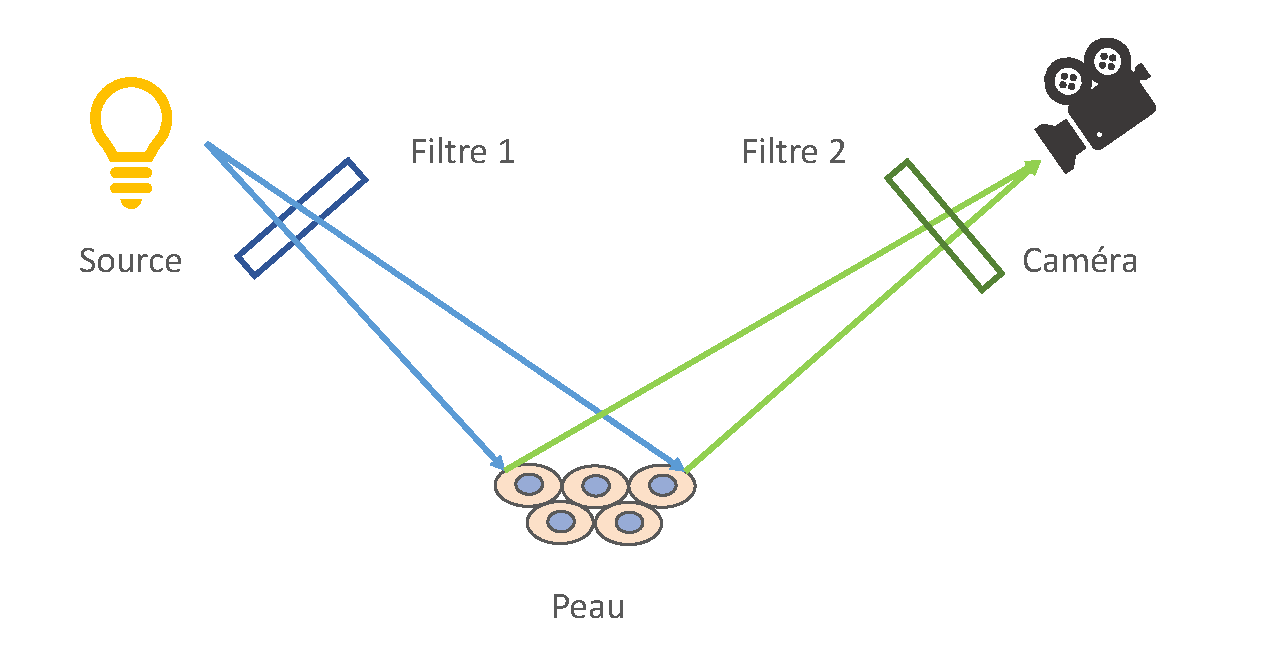
\includegraphics[width=\linewidth]{contents/chapter_2/resources/scheme_multispectral_principle.pdf}
    \caption{Schéma de fonctionnement d'une caméra multispectrale. Ces dispositifs peuvent adapter la longueur d'onde de la source à partir d'éclairage \gls{del}, de lasers ou de filtres (Filtre 1), ou capter différentes longueurs d'onde à partir de la lumière réémise (Filtre 2).}
    \label{fig:scheme_multispectral_principle}
\end{figure}\par

\subsubsection{Microscopie confocale Raman}
Ce type de dispositif porte le nom de l'effet Raman, lui-même inspiré par le nom du physicien Chandrashekhara Venkata Râman à l'origine de cette découverte. Son principe consiste à analyser un décalage de fréquence entre la lumière incidente et la lumière diffusée. Ainsi, ce décalage est propre à chaque matériau et permet de retrouver ce dernier. Cet effet est par son principe non destructif, et a l'avantage de ne pas être dépendant de la longueur d'onde d'excitation. Contrairement à l'effet de fluorescence pour lequel la lumière doit posséder une longueur d'onde spécifique afin d'entrer en \textit{résonance} avec la matière traversée, l'effet Raman s'obtient quelle que soit la longueur d'onde de la lumière. Les différentes interactions et leurs différences sont schématisées sur la \Cref{fig:scheme_principle_raman}.\par

\begin{figure}[H]
    \centering
    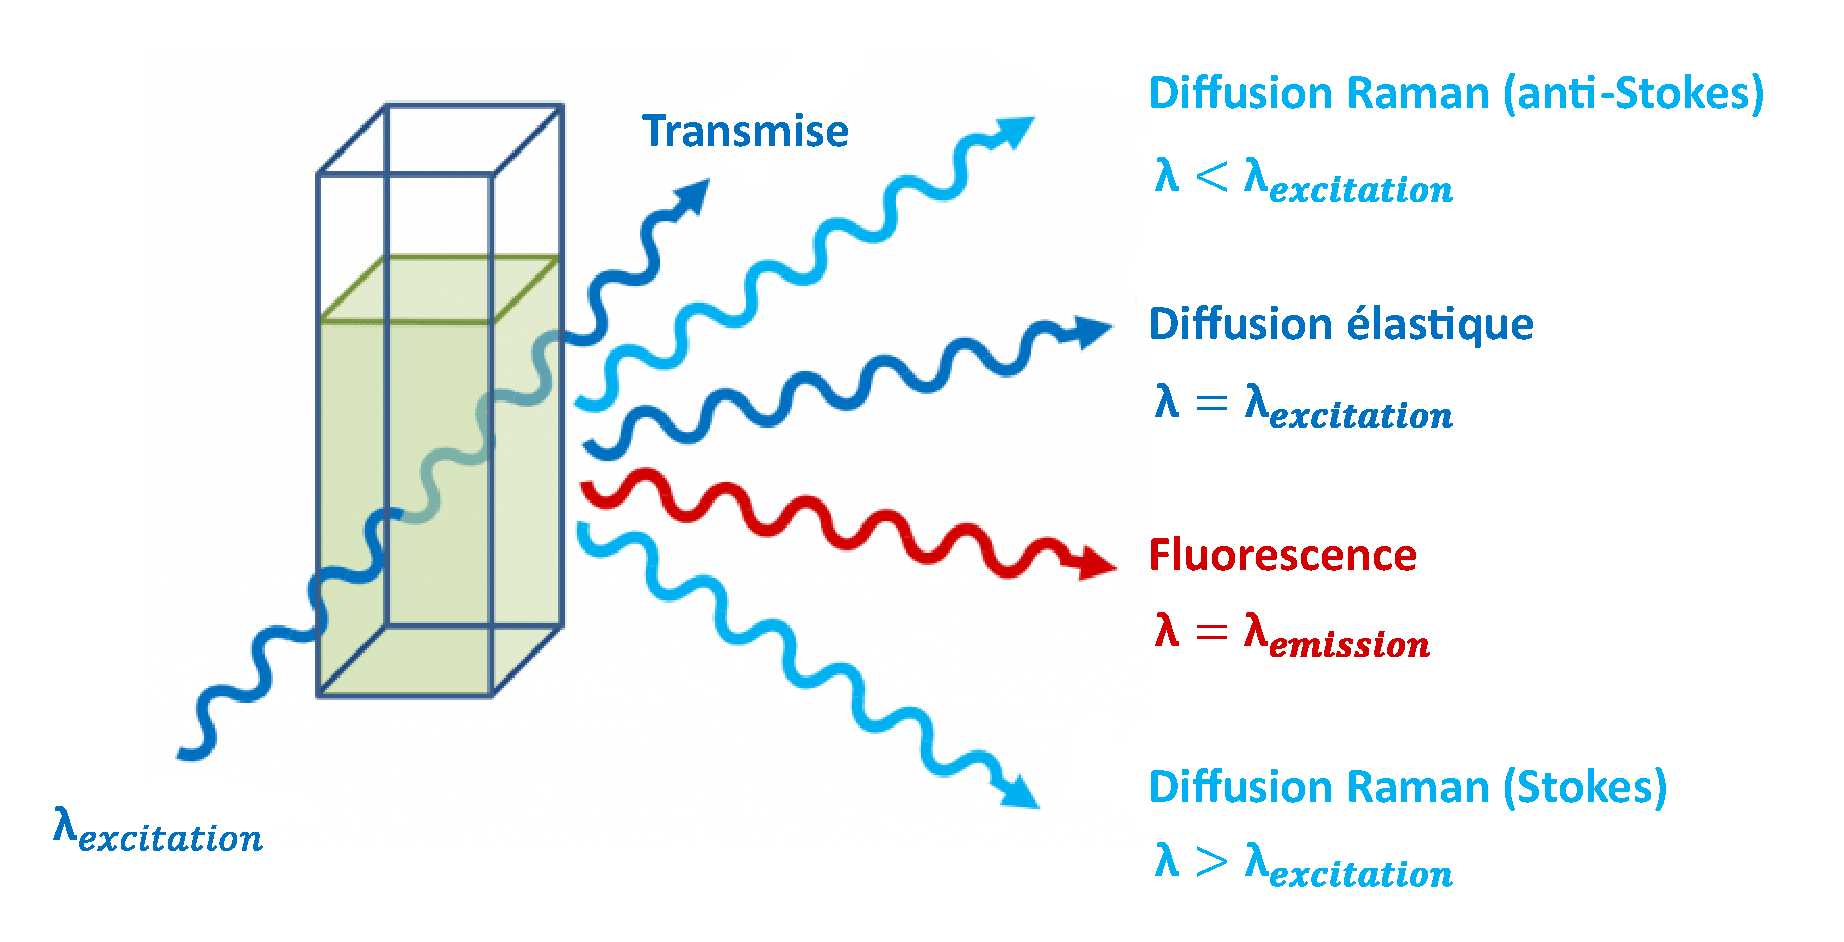
\includegraphics[width=\linewidth]{contents/chapter_2/resources/scheme_principle_raman.pdf}
    \caption{Schéma reprenant les divers effets résultant de l'interaction entre la lumière et la matière\textsuperscript{\ref{footnote:edinburgh_instruments}}. La diffusion Raman se distingue par un décalage de longueur d'onde supérieur (Stokes) ou inférieur (anti-Stokes).}
    \label{fig:scheme_principle_raman}
\end{figure}\par

\addtocounter{footnote}{1}
\footnotetext[\thefootnote]{Source~:~Edinburgh Instruments, Livingston, Royaume-Uni. \label{footnote:edinburgh_instruments}}

Cet effet a été employé en spectroscopie assez tôt~\cite{Ferraro2003} et s'est étendu progressivement à la microscopie confocale~\cite{Caspers2003} permettant d'obtenir non plus une information relative à un point unique, mais d'obtenir des images à deux dimensions, avec une profondeur ajustable par modification du plan focal.\par

Ses applications dans le milieu de la dermatologie sont variées. En effet, de nombreux travaux ont porté sur la détection des lésions cancéreuses mélanocytaires, dont essentiellement le mélanome avec une sensibilité supérieure à 90~\%~\cite{Lui2012,Schleusener2015}. Les lésions cancéreuses non mélanocytaires ont également été abordées dont essentiellement les pathologies de \gls{cbc} et de \gls{csc} avec des précisions de détection élevées, supérieures à 90~\%~\cite{Lieber2008,Silveira2015}.\par
\clearpage

\subsection{Modalités par mesure non-optique}
Cette seconde sous-section se dédie aux modalités d'imagerie offrant une alternative aux techniques optiques employées dans le milieu de la dermatologie. Dans un premier temps, le fonctionnement de l'\gls{irm} est décrit puis dans un second temps celui de l'échographie haute fréquence.\par

\subsubsection{Imagerie par résonance magnétique}
Le principe global de fonctionnement de l'\gls{irm} est basé sur l'interaction et l'observation des moments magnétiques des noyaux d'hydrogène. À leur état initial, les noyaux d'hydrogène possèdent un moment magnétique non contraint et donc désordonné (la somme de ces moments magnétiques à l'échelle macroscopique est approximativement nulle). Ainsi, la première étape consiste à contraindre le moment magnétique des noyaux d'hydrogène dans une même direction (mais pas forcément un même sens) par un champ magnétique constant, on parle de précession. Dans une seconde étape, des radio-fréquences sont émises pour contraindre, de manière homogène, ces moments magnétiques dans une nouvelle direction (généralement perpendiculairement à ce champ) et ce par excitation. Enfin, l'émission de radio-fréquences est stoppée, puis le temps de retour à l'équilibre est mesuré (temps de relaxation) à l'aide d'une antenne de réception. Ce fonctionnement est résumé à l'aide du schéma disponible sur la ~\Cref{fig:scheme_principle_mri}.\par

\begin{figure}[H]
    \centering
    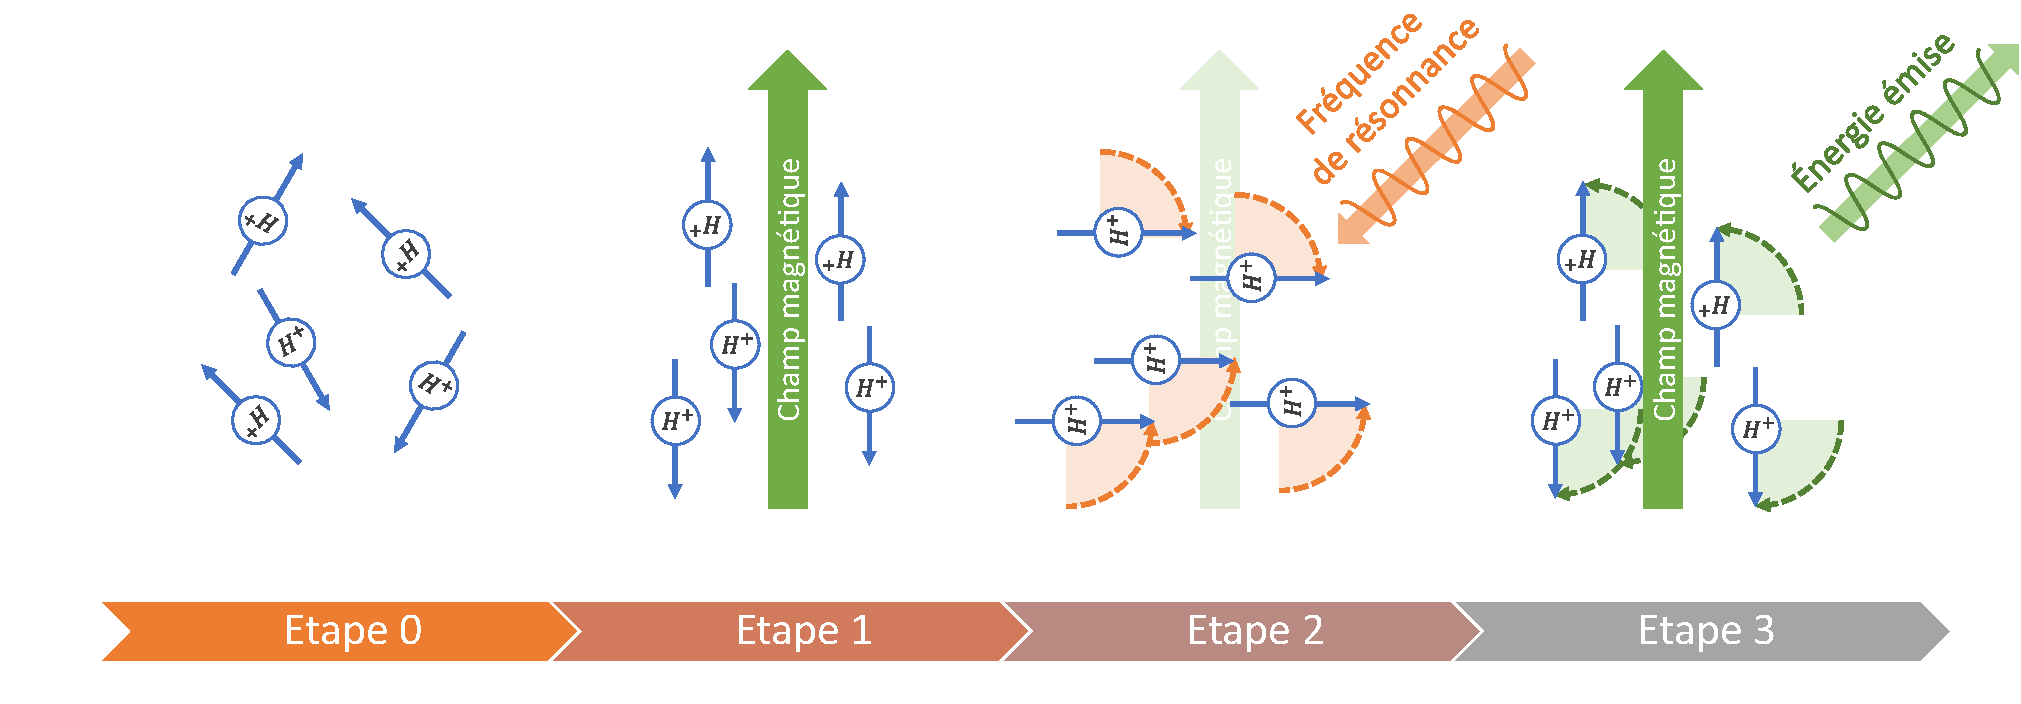
\includegraphics[width=\linewidth]{contents/chapter_2/resources/scheme_principle_mri.pdf}
    \caption{Schéma du principe de fonctionnement de l'\gls{irm} en quatre étapes. Le champ magnétique constant permet de contraindre les noyaux d'hydrogène, puis l'excitation par radio-fréquence permet d'observer par la suite leur temps de relaxation.}
    \label{fig:scheme_principle_mri}
\end{figure}\par

En ce qui concerne l'utilisation de l'\gls{irm} en dermatologie, le champ d'application semble assez restreint, malgré des études positives concernant son utilisation dans le cadre d'actions de dépistage et de son utilisation à but pré-opératoire du mélanome. De plus, l'utilisation d'agents de contraste comme le gadolinium semble être opportun pour le dépistage de lésions de la peau~\cite{Zemtsov1993}. Une étude plus récente liée à la dermatologie a été menée sur les mécanismes nerveux de récompense associés aux démangeaisons, mais implique l'utilisation de l'\gls{irm} fonctionnelle sur la zone du cerveau et non de la peau en elle-même~\cite{Mueller2017}. Néanmoins, l'une des principales contraintes évoquée concerne l'acquisition d'échantillons de faible taille sur des machines conventionnelles rendant le ratio signal sur bruit important et les temps d'acquisition pour compenser ce dernier inexploitable~\cite{Gobel2016}. De plus, les forts coûts associés à ces appareils et leur utilisation contraignante en font des outils difficilement applicables au domaine de la dermatologie.\par

\subsubsection{Échographie haute fréquence}
Les dispositifs d'échographie sont des appareils d'imagerie basés sur l'utilisation d'ondes acoustiques. Pour cela, une sonde composée de transducteurs électro-acoustiques est employée pour l'émission mais également la réception de ces ondes, par utilisation de l'effet piézoélectrique inverse et direct. Il existe de multiples sondes pouvant émettre à divers intervalles de fréquences et permettant d'atteindre diverses profondeurs. Ces ondes sont ainsi émises par la sonde (effet piézoélectrique inverse) et se propagent au sein des tissus du corps humain, avant d'être partiellement renvoyées à chaque changement de l'impédance de ces tissus. Les ondes renvoyées sont ainsi réceptionnées par la sonde émettrice (effet piézoélectrique direct) et pour former un signal.\par

Comme énoncé, différentes fréquences sont employées selon la profondeur recherchée, de \SIrange{2}{10}{\mega\hertz} pour des structures assez lointaines allant de l'abdomen aux artères, et \SIrange{10}{70}{\mega\hertz} pour des structures plus proches et fines telles que la peau et l'oeil. Ainsi, les travaux de la peau par échographie emploient le terme d'échographie haute fréquence.\par

Les travaux de recherche mêlant dermatologie et échographie avant les années 2000 ont montré une efficacité de la technique afin de suivre l'évolution de mélanomes~\cite{Cammarota1998}. Des travaux plus récents ont permis d'étendre la technique à d'autres pathologies cancéreuses telles que les \gls{cbc}~\cite{Barcaui2014}, mais également des \gls{csc}~\cite{Catalano2010}. Enfin, cette technique aurait un potentiel pour le suivi de pathologies plus bénignes telles que l'eczéma ou l'arthrose psoriasique~\cite{Bhatta2018}.\par

\begin{figure}[H]
    \centering
    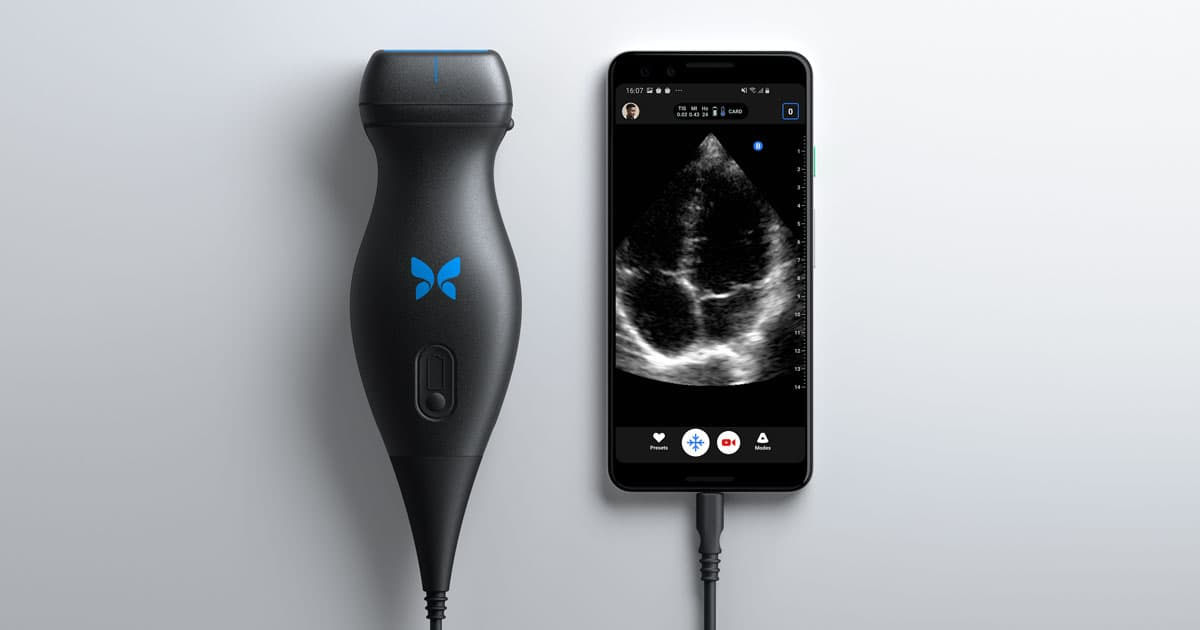
\includegraphics[width=\linewidth]{contents/chapter_2/resources/exemple_ultrasound.jpg}
    \caption{Exemple de la sonde à ultrasons Butterfly iQ\textsuperscript{\ref{footnote:device_ultrasound}}, proposant une solution nomade et connectée.}
    \label{fig:exemple_ultrasound}
\end{figure}\par

\addtocounter{footnote}{1}
\footnotetext[\thefootnote]{Source~:~Butterfly Network, New York, États-Unis. \label{footnote:device_ultrasound}}